\chapter{Implementacja symulacji}
\label{cha:implementacja}

\section{Opis problemu}
\label{sec:opis_problemu}
Symulacja gry 3-osobowej będzie przedstawiona jako sześcian. Każdy z jego wierzchołków będzie miał współrzędną składającą się z kombinacji 0 i 1, co ma obrazować prawdopodobieństwo gracza. Odpowiednio prawdopodobieństwo gracza pierwszego przedstawia oś x, drugiego oś y, trzeciego oś z. Każda funkcja reprezentuje jedną instancję gry 3-osobowej. Rysowane funkcje będą przedstawiały prawdopodobieństwa graczy ($p_i$) wynikające z używanych równań i zachowania przeciwników. 

Symulacja gry N-osobowej, w której gracze ustawieni są w okręgu będzie obrazowana jako funkcje prawdopodobieństwa każdego gracza od numeru partii.
%-------------------------------------------------------------------------------------------------------------------------------------------------------------

\section{Środowisko QT}
\label{sec:qt}
Do stworzenia programu wykorzystano QT Creator IDE z kilku powodów, które zaraz zostaną rozwinięte. Najważniejszą cechą środowiska jest udostępnienie go na kilku rodzajach licencji, z czego użyta tu została licencji LGPL. Pozwala ona na darmowe użytkowanie i modyfikowanie plików źródłowych, lecz udostępnienie własnego programu musi odbyć się na tej samej licencji. Kolejnym ważnym elementem jest multiplatformowość pozwalająca w łatwy sposób przenosić kod programu między systemami operacyjnymi, o ile nie zostały użyte biblioteki dostępne tylko na jeden z systemów. Kolejną z zalet jest łatwy i intuicyjny interfejs tworzenia graficznego interfejsu użytkownika, osoba mająca wcześniej styczność z na przykład biblioteką Swing Java'y nie powinna mieć problemu z zaadaptowaniem się do  formularza QT Creatora. Używanie nowoczesnego języka C++ (w pracy użyto wersji 14) nie sprawia problemów. Przed użyciem klas z bibliotek standardowych C++ warto sprawdzić czy biblioteka QT nie zawiera specjalnych klas opakowujących je. Przykładem może być \texttt{pthread} i \texttt{QThread}.

%-------------------------------------------------------------------------------------------------------------------------------------------------------------

\section{Schemat programu}
\label{sec::schemat}
Rysunek \ref{fig:schemat} przedstawia poglądowy schemat działania programu. Dzieląc rysunek na lewą i prawą część możemy wyodrębnić dwa wątki. Po lewej wątek odpowiadający za wykonanie symulacji, po prawej wątek odpowiadający za rysowanie. Określeniem \textit{Zasób} są opisane współdzielone dane ( opisane w podrozdziale \ref{sec::kod}) między wątkami, którymi jest historia symulacji. 

Podczas startu programu zostaje narysowany sześcian, po czym program przechodzi w stan nasłuchiwania na sygnały. Przykładowymi sygnałami mogą być zmiana rozmiaru okna aplikacji, bądź obrót figury. Po wykryciu takowego, następują próby zablokowania dostępu do zasobu dopóki nie zostanie to wykonane (zasób może być zablokowany przez inny wątek). Następnie na podstawie historii symulacji i/lub sygnału dokonywane jest nowe rysowanie. Po czym zasób zostaje zwolniony, a główny wątek (odpowiedzialny za rysowanie) wraca do stanu nasłuchiwania. 
\begin{figure}
    \centering
    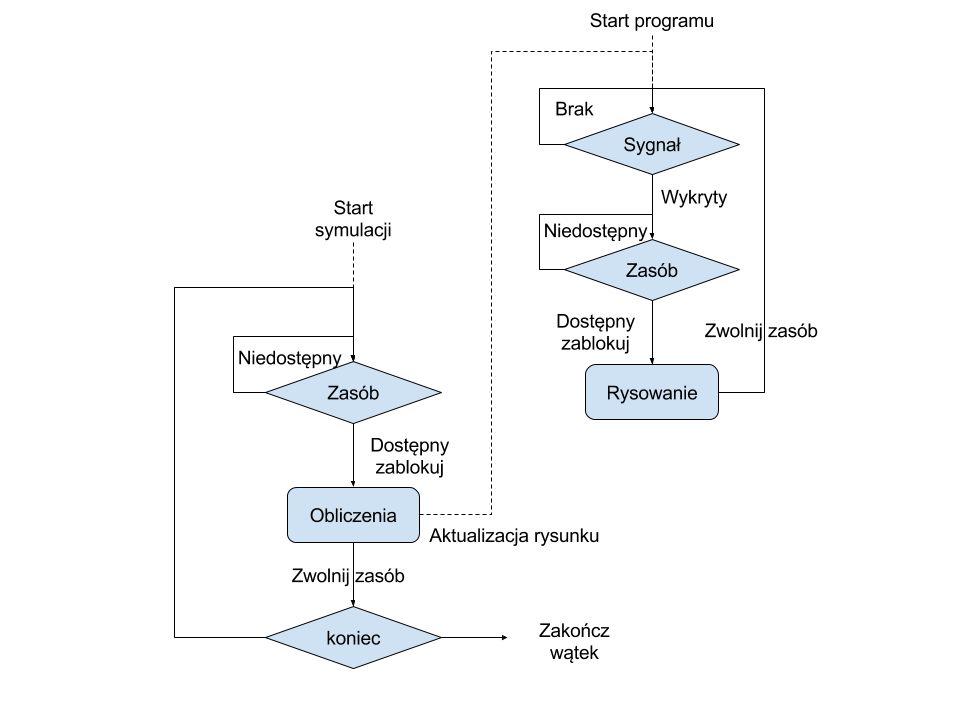
\includegraphics[width=0.9\textwidth]{pict/schemat.png}   
    \caption{Schemat programu}
	\label{fig:schemat} 
\end{figure}
Podczas startu symulacji (spowodowanej naciśnięciem przycisku \texttt{RUN}) identycznie jak poprzednio musi być uzyskany dostęp do zasobów. Dopiero po tym możliwe jest przeprowadzenie symulacji jednej partii dla każdej instancji gry. Następnie wyniki zostają zapisane do zasobów, po czym zasoby zostają zwolnione. Równocześnie do wątku głównego wysyłany jest sygnał mówiący o aktualizacji historii symulacji. Jeśli była to ostatnia planowana partia wątek symulacyjny kończy swoje działanie.
%-------------------------------------------------------------------------------------------------------------------------------------------------------------

\section{Sygnały, sloty i mutex}
\label{sec::sig_slot}
Komunikacja między klasami dziedziczącymi po \texttt{QObject} odbywa się przy pomocy połączonych ze sobą sygnałów i slotów. Można na nie patrzeć jako funkcje (sloty) oraz wskaźniki do funkcji (sygnały). Sygnał może trafiać do wielu slotów oraz do slotu może docierać wiele sygnałów. Ważne jest aby typy parametrów w deklaracji sygnału pokrywały się z typami parametrów deklaracji slotu. W przypadku gdy sygnał będzie miał zbyt dużo parametrów dla slotu, nadmiarowe parametry zostaną pominięte.

W celu uniknięcia kolizji zapis-odczyt na współdzielonych zasobach została użyta klasa \texttt{mutex}. Jest to semafor, nie chroni on danych przed dostępem z wielu źródeł, a jedynie informuje czy zasoby są obecnie używane czy nie. Nie ma niebezpieczeństwa wykonania operacji kolizyjnych, gdyż zasoby są wykorzystywane jedynie przez wewnętrzne struktury programu, które nie wykonują operacji na wspólnych zasobach jeśli semafor jest zablokowany.
%-------------------------------------------------------------------------------------------------------------------------------------------------------------

\section{Kod}
\label{sec::kod}
W tym podrozdziale będą opisane kluczowe fragmenty kodu, niezbędne do zrozumienia implementacji programu. Współdzielonymi zasobami są:
\begin{lstlisting}
template<typename T> using tup3= tuple<T,T,T>;
vector<vector<tup3<double>>> beginsp; //wektor historii punktów początkowych odcinków
vector<vector<tup3<double>>> endsp; //wektor historii punktów końcowych odcinków
vector<tup3<int>>colorsp; //kolory funkcji
mutex points;
\end{lstlisting}

\paragraph{Interfejs klasy \texttt{Game}}
Cała symulacja przeprowadzana jest w klasie \texttt{Game}, dlatego zostanie teraz omówiona. Reprezentuje ona jedną instancję gry 3-osobowej. Parametrem konstruktora jest indeks tablicy \texttt{decision\_funs}, której element zostaje przypisany do \texttt{decision}. \texttt{function} jest wrapperem biblioteki standardowej dla dowolnej funkcji, wyrażenia lambda, wyrażenia bind, funkcjonału lub wskaźników do funkcji. W poniższym kodzie \texttt{function} jest parametryzowany bezargumentowym, bezwynikowym zachowaniem. Funkcja \texttt{next} przeprowadza rozgrywkę jednej partii. Jej implementacja zostanie przedstawiona później. Zmienna \texttt{current} odpowiada $liczba_{partii}$, natomiast \texttt{nr[i]} odpowiada $nast_i$ (opisano w podrozdziale \ref{sec:model}). Funkcja \texttt{checker} jest odpowiednikiem funkcji $ogr$ (opisano w podrozdziale \ref{sec:ograniczenie}). Tablica \texttt{decision\_funs} zawiera funkcje lambda mające dostęp do prywatnych zmiennych klasy \texttt{Game}. W tablicach \texttt{result} znajdują się obliczone $\Delta p_i$, które następnie poddawane są funkcji ograniczającej. 

\begin{lstlisting}
class Game{
public:
    Game(int f);
    tup3<double> next();
    int getCurrent(); //zwraca numer bieżącej partii
    tup3<double> prelast(); //zwraca pre
private:
    array<double,3> p; //prawdopodobieństwa
    tup3<double> pre; //ostatnia krotka prawdopodobieństw na podstawie, których było dokonane losowanie sojuszników
    int current; //numer bieżącej partii
    array<int,3> nr;
    double checker(double r);
    function<void()> decision; //dokonuje modyfikacji prawdopodobieństw
    array<function<void()>,2>decision_funs={{
      [this](){//standardowe
        array<double,3> result= {
            0.1*( 1 - static_cast<double>(nr[1])/current - static_cast<double>(nr[2])/current),
            0.1*( 1 - static_cast<double>(nr[2])/current - static_cast<double>(nr[0])/current ),
            0.1*( 1 - static_cast<double>(nr[0])/current - static_cast<double>(nr[1])/current )
        };
        for(int i=0; i<3; i++)
            p[i]= checker(p[i]+result[i]);
      },
      [this](){//replikatorów
        array<double,3> result= {
            0.1*(p[0]*(1-p[0])*(1-static_cast<double>(nr[1])/current-static_cast<double>(nr[2])/current)),
            0.1*(p[1]*(1-p[1])*(1-static_cast<double>(nr[0])/current-static_cast<double>(nr[2])/current)),
            0.1*(p[2]*(1-p[2])*(1-static_cast<double>(nr[0])/current-static_cast<double>(nr[1])/current))
        };
        for(int i=0; i<3; i++)
            p[i]= checker(p[i]+result[i]);
      }
    }};
};
\end{lstlisting}

\paragraph{Implementacja \texttt{Game::next}}
Tablica \texttt{choices} zawiera losowe wartości dla każdego z zawodników, na podstawie których dokonywane jest losowanie sojusznika.
\begin{lstlisting}
tup3<double> Game::next(){
    pre= make_tuple(p[0],p[1],p[2]);
    current++;
    array<double,3> choices= {static_cast<double>(rand())/RAND_MAX, static_cast<double>(rand())/RAND_MAX, static_cast<double>(rand())/RAND_MAX};
    for(int i=0; i<3; i++)
        if(choices[i]<p[i])
            nr[i]++;
    decision();
    return make_tuple(p[0],p[1],p[2]);
}
\end{lstlisting}

\paragraph{Implementacja wątku symulującego} \texttt{QtConcurrent::run} jest funkcją uruchamiającą w osobnym wątku funkcję podaną jako parametr. Zwraca ona obiekt \texttt{QFuture}, który nie może przerwać lub wstrzymać wątku. Poprzez \texttt{beginsp.resize(p)} tworzony jest wektor posiadający p pustych elementów(wektorów krotek), ponieważ już w pierwszej partii będziemy potrzebować osobnego wektora dla każdej instancji gry. Natomiast \texttt{beginsp[i].reserve(g)} rezerwuje pamięć dla g partii, gdyby ta funkcja nie została użyta prawdopodobnie wystąpiłaby realokacja pamięci, w celu zapewnienia jej ciągłości. Przekładałoby się to na spowolnienie działania programu. Napisałem prawdopodobnie, ponieważ standard języka nie precyzuje ilości pamięci domyślnie rezerwowanej przez wektor, co jest zostawione po stronie implementacji. Przed wykonaniem każdej partii wątek czeka na dostęp do zasobu. Funkcja \texttt{try\_lock()} zwróci \texttt{true} w przypadku udanego przydzielenia zasobu, w przeciwnym razie zwróci \texttt{false}. 
\begin{lstlisting}
QtConcurrent::run(
            [&]()->void{
                ui->pushButton_Run->setEnabled(false);
                const int g= nr_rounds;
                const int p= nr_players;
                const int f= fun;
                vector<unique_ptr<Game>> tab;
                std::default_random_engine generator;
                std::uniform_int_distribution<int> distribution(0,255);
                auto r= bind(distribution, generator);
                clear_vectors();
                chrono::milliseconds d(delay);
                beginsp.resize(p);
                endsp.resize(p);
                for(int i=0; i<p;i++){
                    tab.push_back(make_unique<Game>(f));
                    colorsp.push_back(make_tuple( r(), r(), r() ));
                    beginsp[i].reserve(g);
                    endsp[i].reserve(g);
                }
                for(int j=0; j<g;j++){
                    if(quit) return;
                    while(!points.try_lock());
                    for(int i=0; i<p;i++){
                        beginsp[i].push_back(tab[i]->next());
                        endsp[i].push_back(tab[i]->prelast());
                    }
                    points.unlock();
                    emit copy();
                    this_thread::sleep_for(d);
                }
                ui->pushButton_Run->setEnabled(true);
            });
\end{lstlisting}

%-------------------------------------------------------------------------------------------------------------------------------------------------------------

\section{Rysowanie 3D}
\label{sec::3d}
\paragraph{Rysowanie}
Rysowanie sześcianu oraz funkcji zostało wykonane jako rysowanie odcinków. Ze względu na ograniczony krok czasowy symulacji funkcje wyglądają na wygładzone. Środek sześcianu jest środkiem układu współrzędnych.
\paragraph{Rozszerzanie}
Do rozszerzania ekranu został użyta następująca funkcja:
\begin{lstlisting}
void MyGLWidget::resizeGL(int width, int height){
    int side = qMin(width, height);
    glViewport((width - side) / 2, (height - side) / 2, side, side);
    glMatrixMode(GL_PROJECTION);
    glLoadIdentity();
#ifdef QT_OPENGL_ES_1
    glOrthof(-1, +1, -1, +1, 1.0, 15.0);
#else
    glOrtho(-1, +1, -1, +1, 1.0, 15.0);
#endif
    glMatrixMode(GL_MODELVIEW);
}
\end{lstlisting}
Oknem widgetu jest widoczny na ekranie prostokąt. Oknem roboczym widgetu jest obszar, na którym przeprowadzane są operacje. Oba okna nie muszą się pokrywać, mogą istnieć sytuacje, w których rysowane są elementy poza widokiem użytkownika. Posiadając żądane wymiary nowego okna należy wyznaczyć nowe położenie i wymiary nowego okna roboczego tak, aby zachować proporcje sześcianu oraz przedstawić go w całości. Argumentami funkcji \texttt{glViewport} są kolejno: współrzędne x i y lewego dolnego rogu widoku, szerokość i wysokość okna roboczego. Okno robocze musi być dopasowane do najkrótszego wymiaru widgetu, aby figury nie znalazły się poza oknem widgetu. Aby zapewnić wycentrowanie widoku roboczego należy dobrać punkt początkowy okna roboczego (lewy, dolny narożnik). Musi on mieć współrzędną punktu początkowego krótszej krawędzi jako 0, ponieważ chcemy wykorzystać ją całą. Współrzędna punktu początkowego dłuższej krawędzi okna roboczego musi być oddalona od punktu początkowego okna widgetu o połowę niewykorzystanej długości. Prowadzi to do wzoru na punkt początkowy okna roboczego: 
\begin{equation}
p_0=(\frac{1}{2}(\text{szerokość}-min(\text{szerokość}, \text{wysokość}),\frac{1}{2}(\text{wysokość}-min(\text{szerokość}, \text{wysokość}))
\end{equation}
Mając okno robocze o odpowiednich wymiarach zostało tylko przesunięcie układu współrzędnych do centrum okna roboczego przy pomocy funkcji \texttt{glOrtho}.
\paragraph{Obracanie}
\begin{wrapfigure}{rh}{0.2\textwidth}
    \centering
    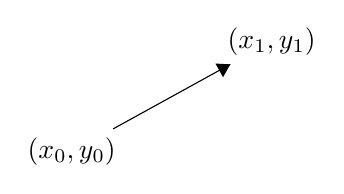
\begin{tikzpicture}[scale=0.2]
		\tikzstyle{every node}+=[inner sep=0pt]
		\draw (34.9,-30) node {$(x_0,y_0)$};
		\draw (47.6,-23) node {$(x_1,y_1)$};
		\draw [black] (37.53,-28.55) -- (44.97,-24.45);
		\fill [black] (44.97,-24.45) -- (44.03,-24.4) -- (44.51,-25.27);
	\end{tikzpicture}
    \caption{Obrót - ruch myszy}
	\label{fig:obrot} 
\end{wrapfigure}
Kąt obrotu figury jest wyznaczany na podstawie punktu, gdzie klawisz myszy został wciśnięty $(x_0,y_0)$ oraz punktu w którym jest nadal wciśnięty $(x_1,y_1)$.
Lewy przycisk myszki ma priorytet nad prawym. Lewy przycisk myszy generuje obrót względem osi x i y o odpowiednio $\Delta$ y i $\Delta$ x stopni, natomiast prawy przycisk generuje obrót względem osi x i z o odpowiednio $\Delta$ y i $\Delta$ x stopni. Obrót jest ograniczony od $0^\circ$ do $360^\circ$, wartości poza tym zakresem są do niego sprowadzane poprzez operacje $\pm 360^\circ$ . Wymnażane delt przez czynnik mniejszy od 1 prowadzi do spowolnienia obrotu.


%-------------------------------------------------------------------------------------------------------------------------------------------------------------

\section{Makefile}
\label{sec::makefile}
Do rysowania wykresu funkcji prawdopodobieństw od numeru partii został użyty plik \texttt{Makefile}, który wykona kompilację, uruchomienie oraz narysowanie wykresu przy pomocy programu gnuplot. Aby uruchomić program należy podać argument: G - ilość partii do rozegrania oraz P - ilość graczy. Poniżej przykładowe polecenie do wykonania symulacji dla 100 partii rozegranych przez 20 zawodników.
\begin{verbatim}
make G=100 P=20
\end{verbatim}
Podanie nierealnych wartości nie da wyniku. Główną różnicą w implementacja gry N-osobowej jest funkcja \texttt{Game::next()}.
\begin{lstlisting}
void Multigame::next() {
    ...
    p[0]+= 0.1*(p[0]*(1-p[0])*(1-static_cast<double>(nr_r[1])/current-static_cast<double>(nr_r[players-1])/current));
    for(int i=1; i<players-1; i++)
        p[i]+= 0.1*(p[i]*(1-p[i])*(1-static_cast<double>(nr_r[i+1])/current-static_cast<double>(nr_r[i-1])/current));
    p[players-1]+= 0.1*(p[players-1]*(1-p[players-1])*(1-static_cast<double>(nr_r[0])/current-static_cast<double>(nr_r[players-2])/current));
}
\end{lstlisting}
Szacowanie prawdopodobieństw musi być wykonane w pętli, ze względu na nieznaną liczę graczy.